%%%%%%%%%%%%%%%%%%%%%%%%%%%%%%%%%%%%%%%%%%%%%%%%%%%%%%%%%%%%%%%%%%%%%%%%%%%%%%%%
%%%%%%%%%%%%%%%%%%%%%%%%%%%%%%%%%%%%%%%%%%%%%%%%%%%%%%%%%%%%%%%%%%%%%%%%%%%%%%%%
%%%%%%%%%%%%%%%%%%%%%%%%%%%%%%%%%%%%%%%%%%%%%%%%%%%%%%%%%%%%%%%%%%%%%%%%%%%%%%%%
\chapter{Marco teórico}
\label{cha:theo}
%%%%%%%%%%%%%%%%%%%%%%%%%%%%%%%%%%%%%%%%%%%%%%%%%%%%%%%%%%%%%%%%%%%%%%%%%%%%%%%%
%%%%%%%%%%%%%%%%%%%%%%%%%%%%%%%%%%%%%%%%%%%%%%%%%%%%%%%%%%%%%%%%%%%%%%%%%%%%%%%%
%%%%%%%%%%%%%%%%%%%%%%%%%%%%%%%%%%%%%%%%%%%%%%%%%%%%%%%%%%%%%%%%%%%%%%%%%%%%%%%%



\color{dieg}
\color{vero} La forma de describir la dinámica \color{norm} de las partículas es mediante  teorías cuánticas de campos  en un marco teórico en donde estas son campos probabilísticos en el espacio--tiempo junto con una coordenada extra de espín.
Cada partícula es un campo que tiene ciertas interacciones con otros campos y con el espín.%; se dice que los fermiones conforman la materia, y los bosones median las interacciones.
\color{norm}


El \color{vero} Modelo Estándar de Física de Partículas, \stdmod, \color{norm} se constituye de un conjunto de partículas (campos), \color{vero}las  interacciones \color{norm} entre las mismas (también campos); que junto con unos ciertos acoplos y parámetros (véase Tabla \ref{tab_stdparams}) dan lugar a uno de los modelos más consistentes y precisos de la naturaleza.

\begin{table}[H]
\centering
\begin{tabular}{lc}
\toprule
Descripción & Parámetros \\ \midrule
Constantes de acoplo \textit{\emph{gauge}} & 3\\
Parámetros del potencial escalar & 2 \\
Masas de $\mathrm{e^-}$, ${\upmu^-}$ y ${\uptau^-}$ & 3 \\
Masas de los 6 quarks & 6\\
Fases físicas de la matriz  \textsc{ckm}  & 3 \\
Fase de violación CP & 1\\
Parámetro de CP de la fuerza fuerte & 1\\ \midrule
Total & 19\\
\bottomrule
\end{tabular}
\caption{Los 19 parámetros del \stdmod, de los cuales 4 provienen de la matriz \textsc{ckm}. Estos parámetros no son predichos por el \stdmod, deben ser medidos o determinados mediante experimentos.}	\label{tab_stdparams}
\end{table}
%
\color{norm} 
%
%
Varios de esos parámetros nacen de la teoría de Kobayashi--Maskawa \cite{km1}, propuesta en 1973, y que predecía la existencia de una tercera generación de dobletes de quarks (véase Figura \ref{fig:1a}), pudiendo los quarks mezclarse atendiendo a la matriz de Cabibbo--Kobayashi--Maskawa (CKM)  y que fue \color{vero} apoyada \color{norm} en 1977 con la primera observación del mesón $\Upsilon [\mathrm{b\bar{b}}]$.
%

%En el \stdmod la violación CP \color{vero} se describe \color{norm} con una matriz $3\times3$, unitaria y con una fase irreducible: la matriz CKM. La existencia de las familias de quarks y leptones dan lugar a varios de los parámetros del \stdmod, entre ellas las masas y los \color{vero} elementos de la matriz CKM. \color{norm}
%%
%La violación de la simetría CP implica que, en resumidas cuentas, materia y antimateria se comporta de un modo diferente, y la prueba más evidente de ellos es la propia asimetría que hay en el Universo entre ambas.
%%
%En las desintegraciones débiles se violan tanto P como C por separado, pero es más transcendente todavía que se viole CP, puesto que ello permite definir de modo absoluto que es materia y que es antimateria. 
%%Isto ocorre, por exemplo, na desintegración semileptónica do mesón K0L que decae con maior frecuencia a positróns.
%La violación CP es algo verdaderamente desconcertante, puesto que en el mundo macroscópico no se ve ninguna razón por la que derecha e izquierda deban de tener un significado absoluto en la naturaleza. No tiene que ver exactamente con un cambio de sentido, sino más bien con una reflexión especular y el cambio de partícula por antipartícula, es decir, el cambio de un sistema de referencia levógiro por uno dextrógiro.

% top lifetime
%La vida media tan corta del quark \emph{top}, $t$, no permite que este forme mesones y el siguiente quark más pesado es el $b$ --- el más ligero de la familia y que sí forma hadrones. Por este último motivo, los hadrones con $b$ decaen a otras familias en términos de los parámetros de la matriz CKM, y es en estas desintegraciones débiles, mediante diagramas de caja o con \emph{loops}, donde aparecen asimetrías CP observables y de gran interés.



%%%%%%%%%%%%%%%%%%%%%%%%%%%%%%%%%%%%%%%%%%%%%%%%%%%%%%%%%%%%%%%%%%%%%%%%%%%%%%%%
\section{El Modelo Estándar} %%%%%%%%%%%%%%%%%%%%%%%%%%%%%%%%%%%%%%%%%%%%%%%%%%%

El Modelo Estándar es una teoría cuántica de campos (QFT) no abeliana (dícese de Yang--Mills) que describe tres de las cuatro interacciones fundamentales de la naturaleza, nombradamente: nuclear fuerte, nuclear débil y electromagnética.
Estas interacciones se asocian con simetrías \emph{gauge} y a los mediadores de dichas interacciones se les conoce como bosones \emph{gauge} \cite{pdg2018}.

La interacción fuerte es descrita por la Cromodinámica Cuántica (QCD, \emph{Quantum Chromodynamics}), y se corresponde con un grupo de simetría $SU(3)_{C}$, de carga de color $C$. Por otra parte, las interacciones electromagnética y débil se describen conjuntamente con la teoría Electrodébil (EW, \textit{ElectroWeak}), de simetría $SU(2)_T \otimes U(1)_Y $ de isospín débil $T$ e hipercarga $Y$. Por lo tanto la simetría \emph{gauge} del \stdmod es 
\[SU(3)_{C}\otimes SU(2)_T \otimes U(1)_Y \]
y es rota espontáneamente por el valor de esperanza en el vacío (VEV) de la componente neutra de un doblete escalar de isospín con hipercarga $\sfrac{1}{2}$, denominado bosón de Higgs (véase \S \ref{sec_higgsmecha}),
\begin{equation}
	SU(3)_{C}\otimes SU(2)_T \otimes U(1)_Y -\!\!\!\!-\!\!\!\overset{\mathrm{H^0}}{-\!\!-}\!\!\!\rightarrow SU(3)_C \otimes U(1)_{\text{EM}}.
\end{equation}
Como resultado de esta ruptura de simetría, se combinan los bosones EW en $\mathrm{W^{\pm},\, Z^{0}}$ y $\upgamma$; así como también aparecen las masas de los fermiones al estos interaccionar con el Higgs.



%%%%%%%%%%%%%%%%%%%%%%%%%%%%%%%%%%%%%%%%%%%%%%%%%%%%%%%%%%%%%%%%%%%%%%%%%%%%%%%%

\subsection{Partículas elementales} %%%%%%%%%%%%%%%%%%%%%%%%%%%%%%%%%%%%%%%%%%%%

El \stdmod divide las partículas elementales en dos bloques según las propiedades radicalmente distintas que estas presentan: fermiones de espín semientero, y bosones de espín entero. \color{vero} Ocurre esto también con las partículas compuestas,  los hadrones que son estados ligados de quarks y gluones. \color{norm} Por adición de espín también se clasifican en estos bloques, por ejemplo: los mesones (estados $q-\bar{q}$, como el $\Bs$) son bosones, mientras que los bariones (compuestos de tres quarks, como el protón) son fermiones.


\subsubsection{Fermiones} %

El sector de los fermiones se reparte entre quarks y leptones, cuya principal diferencia radica en que estos últimos no sienten la interacción fuerte. 
La interacción fuerte \color{vero} actúa \color{norm} con los quarks haciendo que estos existan en uno de los tres posibles estados, que se identifican por su carga de color.

En términos de carga \color{vero} se clasifican \color{norm} como:  de carga $+\sfrac{2}{3}$, los quarks u (\emph{up}), c  (\emph{charm}) y t (\emph{top/truth}); de carga $-\sfrac{1}{3}$, los quarks $\mathrm{d}$ (\emph{down}), $\mathrm{s}$ (\emph{strange}) y $\mathrm{b}$ (\emph{bottom/beauty}); de carga $0$, los leptones $\upnu_{\text{e}}$ (neutrino electrónico), $\upnu_{\upmu}$ (neutrino muónico) y $\upnu_{\uptau}$ (neutrino tau); y de carga $-1$, los leptones $\text{e}$ (electrón), $\upmu$ (muón) y $\uptau$ (tau).

Así mismo, existen las llamadas familias para quarks y leptones, tres para cada tipo, de forma que las interacciones fuerte y electrodébil son iguales para cada familia. La primera familia de quarks (leptones) es la formada por $\mathrm{u,d}$ ($\text{e},\upnu_e$), la segunda $\mathrm{c,s}$ ($\upmu,\upnu_{\upmu}$) y la tercera se corresponde con $\mathrm{t,b}$ ($\tau,\upnu_{\uptau}$).



\subsubsection{Bosones} %

\color{dieg}
Los bosones de las \color{vero} Figuras \ref{fig:1c} y \ref{fig:1d} \color{norm} son partículas elementales de espín entero, y que se asocian con las interacciones fundamentales del \stdmod. De estos, los bosones con espín \color{vero} $1$ \color{norm} son los bosones \emph{gauge}, y median las interacciones; mientras que solo el bosón de Higgs carece de espín. \color{norm}
  
Los bosones \emph{gauge} son: el fotón ($\upgamma$), es el mediador de la interacción electromagnética (E) y carece de masa; los bosones $\mathrm{W^+}$, $\mathrm{W^-}$ y $\mathrm{Z^0}$, son los responsables de la interacción débil (W) y tienen masas elevadas: los bosones $\mathrm{W^{\pm}}$ aparecen en transiciones con corrientes cargadas (CC), mientras que las corrientes neutras (NC) proceden vía $\mathrm{Z^0}$; los gluones ($\mathrm{g}$), median la interacción fuerte careciendo de masa.
%
\color{dieg}
Finalmente, el bosón de Higgs \color{vero} confiere  masa a las partículas del \stdmod, tanto a los fermiones como a los bosones \emph{gauge} y a sí mismo. \color{norm}


\begin{figure}[H]
\centering
\subfloat[Los 6 quarks en sus 3 generaciones, I, II y III  columna; y sus 2 familias, I y II fila.\label{fig:1a}]{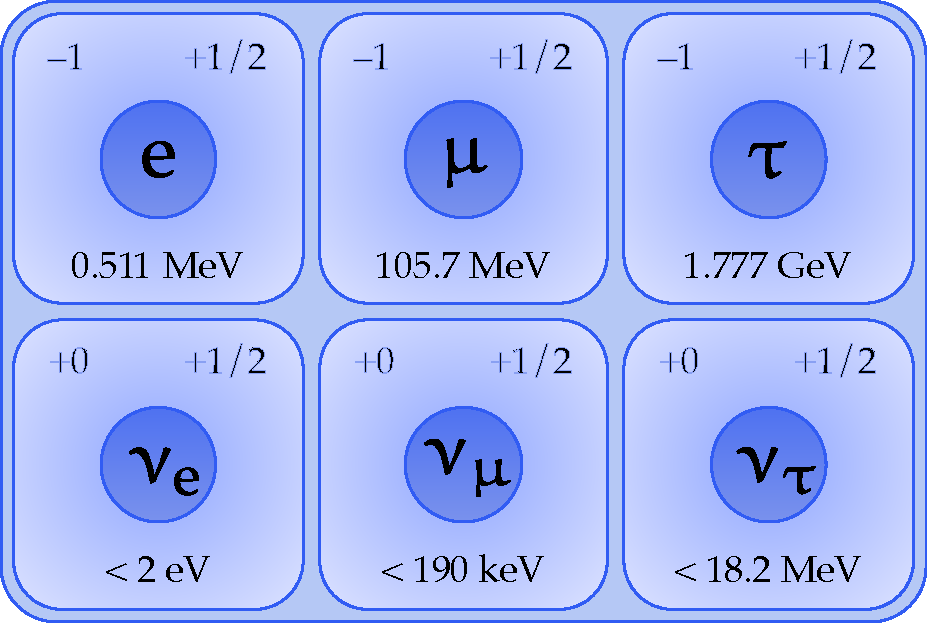
\includegraphics[scale = 0.3]{Leptons.pdf}} \phantom{olaola}
\subfloat[Los 6 leptones en sus 3 generaciones, I, II y III  columna; y sus 2 familias, I y II fila.\label{fig:1b}]{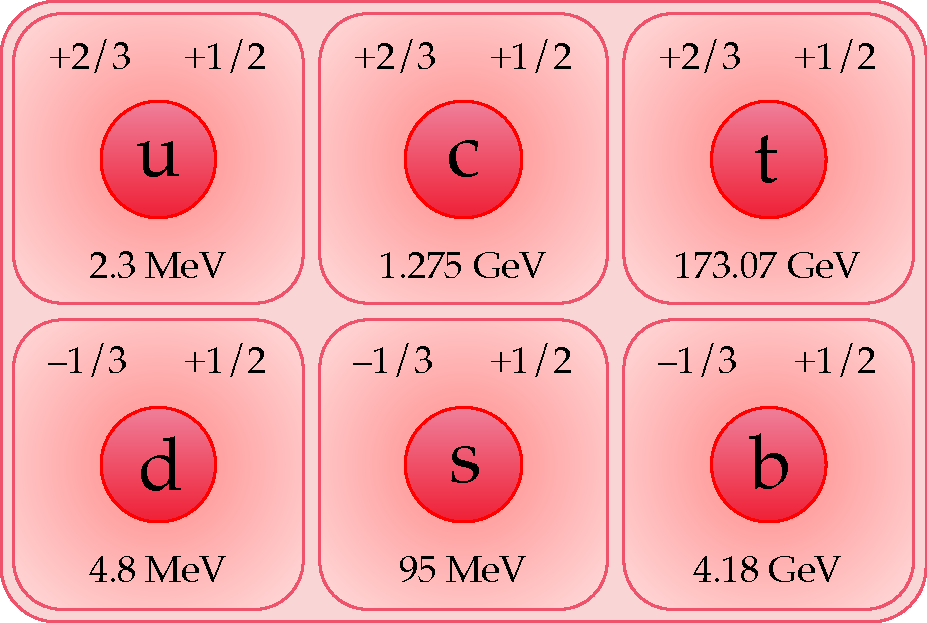
\includegraphics[scale = 0.3]{Quarks.pdf}}\\
%
\subfloat[Bosones \emph{gauge}, portadores de las interacciones.\label{fig:1c}]{\phantom{ola}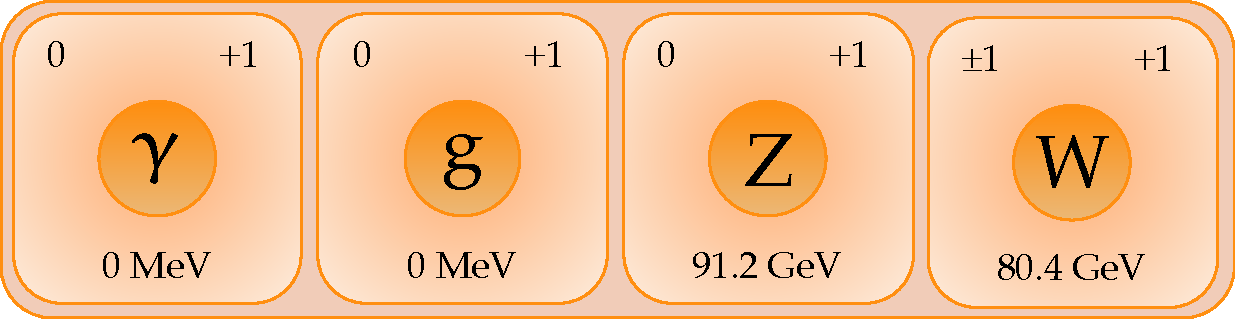
\includegraphics[scale = 0.3]{Bosons.pdf}}\phantom{ola}
\subfloat[Bosón de Higgs.\label{fig:1d}]{\phantom{ola}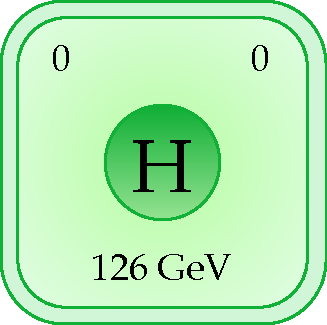
\includegraphics[scale = 0.3]{Higgs.pdf}\phantom{ola}}
\caption{Partículas del \stdmod, los fermiones en las Figuras (a) y (b); y los bosones en las Figuras (c) y (d). En cada cuadro puede verse la carga (arriba izquierda), espín (arriba derecha) y la masa (abajo).} \label{stdmod_particles}
\end{figure}


\color{new}
%%%%%%%%%%%%%%%%%%%%%%%%%%%%%%%%%%%%%%%%%%%%%%%%%%%%%%%%%%%%%%%%%%%%%%%%%%%%%%%%
\subsection{Simetrías discretas en el \stdmod} %%%%%%%%%%%%%%%%%%%%%%%%%%%%%%%%%

La correlación del espín con el espacio--tiempo provoca que existan diferentes estados de una misma partícula. Por ejemplo, se dice que existen fermiones a izquierdas (\emph{left--handed}) o a derechas (\emph{right--handed}), y el operador de paridad, $\OPp$, cambia de una a la opuesta invirtiendo las coordenadas espaciales, es decir, cambiando su helicidad. Aparte del operador $\OPp$, existen otros dos más de transcendental importancia, $\OPc$ y $\OPt$, que se describen a continuación. 



%%%%%%%%%%%%%%%%%%%%%%%%%%%%%%%%%%%%%%%%%%%%%%%%%%%%%%%%%%%%%%%%%%%%%%%%%%%%%%%%
\paragraph{Operador $\bm{\mathsf{\OPt}}$}

La transformación de inversión temporal en física clásica consiste en hacer el cambio $ t \rightarrow - t$; es decir, invertir el sentido del tiempo. Las leyes de la física clásica son  invariantes frente a esta transformación, y en un principio se consideraba que esta era una  simetría verificada de forma exacta por todas las interacciones fundamentales conocidas; de modo que la evidente asimetría temporal en el mundo  macroscópico se atribuía a la muy diferente probabilidad de las configuraciones  macroscópicas iniciales y finales en la evolución de los sistemas. 
%
En la Mecánica  Cuántica hay que encontrar un operador $\OPt$ adecuado para la inversión temporal. Un sistema será simétrico bajo $\OPt$ cuando $[ \OPt, \mathcal{ H}] = 0$ y la función de onda $\OPt \psi$ satisfaga la misma ecuación de  Schrödinger que $\psi$, lo que se traduce en que $\OPt \psi ( t) \neq \psi (- t) = \psi (\bar{ t})$.
%
La transformación correcta de la función de onda bajo el operador $\OPt$ resulta ser $\OPt \psi ( t) = \psi^* (\bar{ t})$, por lo que el operador $\OPt$ es  antiunitario; ello implica que no existen  autoestados del operador $\OPt$, y por lo tanto tampoco números  cuánticos asociados.
%
La interpretación más física de la acción de $\OPt$ es la inversión del movimiento, inviertiendo tanto el momento  linear como el angular.



\paragraph{Operador $\bm{\OPcp}$}

El operador $\OPcp$ se compone de la acción del operador conjugación de carga, $\OPc$, y del operador de paridad, $\OPp$.
%\[ \mathcal{P} |\vec{r}, \vec{p}, \vec{J} \rangle =  |-\vec{r}, -\vec{p}, \vec{J} \rangle  \]
%\[\mathcal{C} | Q, A, L ,S ,C, B, T,  I^3, \vec{p} , \vec{s} \rangle = | -Q, -A, -L ,-S ,-C, -B, -T,  -I^3, \vec{p} , \vec{s} \rangle,\]
%donde 
El operador de paridad invierte las coordenadas espaciales, cambiando de signo la posición y el momento lineal, mientras que mantiene los momentos angulares. Por otra parte, el operador de conjugación de carga mantiene intactas las magnitudes dinámicas, cambiando el signo de los números  cuánticos aditivos: $ Q$, la carga eléctrica; $A$, el número  bariónico; $ L$, el número  leptónico; $I^3$, la tercera componente de  isospín; y $ S, C, B, T$, los números cuánticos de \textit{strange}, \textit{charm}, \textit{beauty} y \textit{truth}, respectivamente.
%
La violación de la  simetría CP implica, en resumidas cuentas, que materia y  antimateria se comportan de forma diferente, y la prueba más evidente de esta violación de  simetría es la preponderancia que existe en el Universo entre materia y  antimateria. En las desintegraciones débiles se violan tanto P como C por separado, pero es mucho más trascendente que  se viole CP, puesto que nos permite definir de manera absoluta qué es materia y qué es  antimateria. Esto ocurre, por ejemplo, en la desintegración  semileptónica del mesón $ K_L^0$, que decae con mayor frecuencia a  positrones que a electrones. 
%
%La violación  CP es realmente desconcertante. 
De acuerdo con la experiencia diaria  macroscópica, no se ve ninguna razón por la que derecha e izquierda deban tener un significado absoluto en la naturaleza. La violación CP no tiene que ver exactamente con el cambio de sentido, sino más bien con la reflexión especular y el cambio de partícula por  antipartícula; es decir, con el cambio de un sistema de referencia  levógiro por otro  dextrógiro.%\footnote{La diferencia clave entre una rotación arbitraria en el espacio y una reflexión espacial es que en esta última un sistema de referencia  dextroxiro pasa a ser  levoxiro, y viceversa.}.



\paragraph{Teorema CPT}

Existe un importante teorema global que permite deducir, entre otras cosas, que la masa y la vida media de las partículas tienen que ser iguales a las de sus  antipartículas. Es el teorema CPT, basado en hipótesis muy generales de la Teoría  Cuántica de Campos y de la Relatividad Especial. Establece que todo  Hamiltoniano que sea  invariante bajo transformaciones de  Lorentz y traslaciones en el espacio--tiempo, que obedezca el principio de  microcausalidad y que tenga un espectro energético con un estado de energía mínimo (el vacío) debe ser  invariante también bajo la acción combinada de los operadores $\OPc$, $\OPp$ y $\OPt$ en cualquier orden. Esto significa que el operador  Hamiltoniano, $\mathcal{ H}$, debe  conmutar con la operación $\OPcp\OPt$; es decir, $[\mathcal{ H},\OPcp\OPt] = 0$.
Aplicar dos veces $\OPcp\OPt$ lleva de nuevo al mismo estado, cuya parte real se corresponde con la masa. Si la partícula es inestable, los autovalores tendrían una parte compleja con información de su anchura y vida media. 
 % y se puede escribir que
%\[ \langle \psi | \mathcal{H} | \psi \rangle = \langle \psi | \mathcal{H} (\mathcal{CPT})^2| \psi \rangle = \langle \psi | \mathcal{CPT} \ \mathcal{H} \ \mathcal{CPT} | \psi \rangle = \langle \overline{\psi} | \mathcal{H} | \overline{\psi} \rangle\]
%donde $\psi$ es el estado correspondiente a una partícula en reposo cuyo  autovalor para el  Hamiltoniano es su masa,  y $\overline{\psi}$ es el estado de su  antipartícula. 
Entonces la  invariancia de $\mathcal{ H}$ frente a $\OPcp\OPt$  predice inmediatamente la igualdad de masa de cada partícula con su  antipartícula.
%Verificar la igualdad de la masa de una partícula y su  antipartícula  es sinónimo de verificar la validez del teorema $\OPcp\OPt$ y de las hipótesis en las que se fundamenta. 
El mejor \textit{test} experimental de la  invariancia $\OPcp\OPt$ en la actualidad lo proporciona la medición de las masas del $ K{}^0$ y del $\overline{ K}{}^0$ (que no son los  autoestados de $\OPcp$): $\left|\frac{ M( K{}^0) -  M(\overline{K}{}^0)}{ M( K{}^0)} \right| \leq 6 \times 10^{-19}$ \cite{pdg2018}.



\color{norm}

\subsection{Lagrangiano} %%%%%%%%%%%%%%%%%%%%%%%%%%%%%%%%%%%%%%%%%%%%%%%%%%%%%%%
\label{sec_yukawa}

Bajo el esquema de partículas de la Figura \ref{stdmod_particles}, se puede construir un lagrangiano, $\mathcal{L}_{\text{\stdmod}}$, que contiene la dinámica de todas las partículas. En él podemos diferenciar la parte relacionada con el bosón de Higgs, $\mathcal{L}_{\text{H}}$, que rompe la simetría $ SU(3)_C \otimes SU(2)_T \otimes U(1)_Y $; y la parte que conserva la simetría, $\mathcal{L}_{\text{FB}}$,
\begin{equation}
\mathcal{L}_{\text{\stdmod}} = \mathcal{L}_{\text{FB}} + \mathcal{L}_{\text{H}}.
\end{equation}
A su vez $\mathcal{L}_{\text{FB}}$ se puede descomponer en las partes correspondientes a quarks (Q), leptones (L) y bosones \emph{gauge} (GB),
\begin{equation}
\mathcal{L}_{\text{FB}} = 3 \mathcal{L}_{\text{Q}} + 3 \mathcal{L}_{\text{L}} + \mathcal{L}_{\text{GB}},	
\end{equation}
y separando las partes cinética ($\mathcal{K}$), que contiene las correspondientes derivadas covariantes que preservan la invariancia \emph{gauge}, y de interacción ($\mathcal{V}$) podemos distinguir
\begin{equation}
\begin{split}
\mathcal{L}_{\text{Q}} &= \mathcal{K}_{\text{Q}} + \mathcal{V}_{\text{Q,EW}} + \mathcal{V}_{\text{Q,S}} \\
\mathcal{L}_{\text{L}} &= \mathcal{K}_{\text{L}} + \mathcal{V}_{\text{L,EW}} .
\end{split}	
\end{equation}

El mecanismo de Higgs, que da masa a las partículas del \stdmod, fue propuesto de modo que las simetrías \emph{gauge} no estuvieran explícitamente rotas. El campo de Higgs rompe la simetría electrodébil de forma espontánea, al tener este un valor de expectación no nulo en el vacío (VEV, véase \S \ref{sec_higgsmecha}). Esta teoría propuesta en la década de los sesenta quedó \color{vero} apoyada \color{norm} en 2012 con el descubrimiento del bosón de Higgs \cite{Aad:2012tfa,Chatrchyan:2012xdj}. Esta parte del lagrangiano la podemos dividir, en consonancia con las anteriores, en
\[\mathcal{L}_{\text{H}} = \mathcal{K}_{\text{H}} + \mathcal{V}_{\text{H,H}} + \mathcal{V}_{\text{H,EW}} + \mathcal{V}_{\text{Y}}\]
siendo $\mathcal{K}$ el término cinemático; $\mathcal{V}_{\text{HH}}$ la interacción consigo mismo y que permite un valor no nulo de $v_0$; $\mathcal{V}_{\text{H,EW}}$ 
que permite dar masa a los bosones $\mathrm{W^{\pm}}$ y $\mathrm{Z^0}$ una vez que se rompe la simetría; y  $\mathcal{V}_{\text{Y}}$ el término de Yukawa que contiene las interacciones fermiónicas que permiten dar masa a los fermiones una vez rota la simetría EW.


\color{new}
\subsection{Mecanismo de Higgs y ruptura espontánea de simetría}
\label{sec_higgsmecha}

Un lagrangiano que contenga tan solo términos de la simetría \emph{gauge} no es suficiente para construir un modelo en el que existan partículas masivas. Si la simetría no se rompe, los bosones carecen de masa; e incluso las masas de los fermiones, bien sean de Dirac o Majorana, también romperían la simetría.
Por otra parte, la simetría $SU(2)_T \otimes U(1)_Y$, que describe la interacción electrodébil, establece una interacción débil que tiene largo alcance, como el electromagnetismo, donde los bosones mediadores tienen masa nula.
Sin embargo, la realidad es bien distinta, puesto que la interacción es de corto alcance 
y está caracterizada por una constante de Fermi,
$G_F$. La simetría \emph{gauge} se encuentra por tanto rota en la naturaleza.


Para explicar este fenómeno se le atribuyó al vacío la
responsabilidad de la ruptura de la simetría, admitiendo la posibilidad de que en él determinados
campos presenten un valor esperado no nulo, lo que vino en llamarse \textit{Electroweak Spontaneous Symmetry Breaking} (EWSSB). Steven Weinberg añadió 4 campos escalares reales de espín cero a la teoría EW $SU(2)_T \otimes U(1)_Y$, dos de ellos con carga ($\phi_1^+$ y $\phi_2^+$) y otros dos neutros ($\phi_3^0$ y $\phi_4^0$), en la forma de un doblete escalar de isospín débil con $I^3 = \sfrac{1}{2}$
\begin{equation}
  \phi(x) = \begin{pmatrix}
    \phi^+(x) \\ \phi^0 (x) 
  \end{pmatrix} = \frac{1}{\sqrt{2}} \begin{pmatrix}
    \phi_1^+(x) + i\phi_2^+(x) \\ \phi_3^0(x) + i\phi_4^0(x) 
  \end{pmatrix}.
\end{equation}
En esta configuración, las 4 partículas escalares tienen hipercarga
débil $Y = +1$. Al campo $\phi_3^0$
se le obliga a tener un valor esperado en el vacío (VEV), $v_0$, muy
elevado: $\phi_3^0(x) = v_0+ H(x)$.
Para ello se postula que el campo $\phi_3^0 (x)$ se encuentra en autoacoplo, siendo la energía potencial de Higgs 
\begin{equation}
V(\phi) = \mu^2 (\phi^{\dagger} \phi) + \lambda (\phi^+ \phi)^2,  \qquad \text{con } \mu^2<0 \text{ y } \lambda >0
\end{equation}
que tiene un estado de mínima energía que se alcanza cuando el campo (sin partículas) toma el valor constante
\[\phi_0 = \langle 0 | \phi | 0 \rangle = \frac{1}{2} \begin{pmatrix}
  0+i0\\ v_0+ i0
\end{pmatrix}\]
siendo $v_0^2 = \frac{-\mu^2}{2 \lambda} = (246.22 \, \mathrm{GeV})^2$. Dicho potencial y su VEV, que se pueden observar en la Figura \ref{fig_higgspot}, dan origen a una partícula de Higgs de masa $M_{\mathrm{H^0}} = \sqrt{2 \lambda v_0^2}$, carga eléctrica neutra e hipercarga $+1$.  

\begin{figure}[H]
\centering

\color{norm}

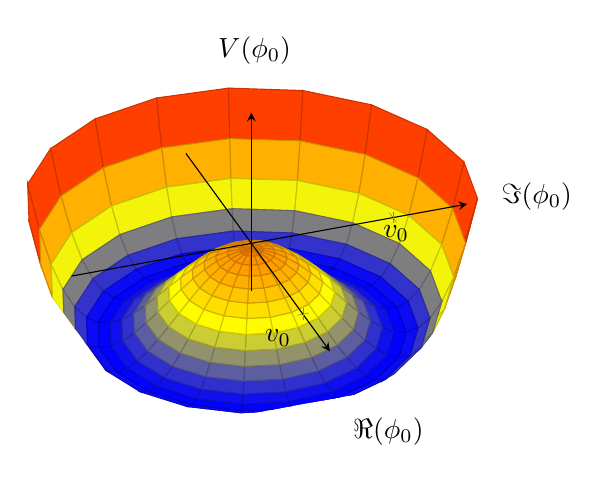
\begin{tikzpicture}
   \begin{axis}[view={70}{30},
                %colormap={blackwhite}{red!50(0cm)=(1); orange(1cm)=(0)},
                axis lines=middle,axis on top,
                xlabel=$\Re(\phi_0)$,ylabel=$\Im(\phi_0)$,zlabel=$V(\phi_0)$,
                x label style={at={(axis description cs:0.625,0.0)},anchor=west},
                y label style={at={(axis description cs:0.9,0.525)},anchor=west},
                z label style={at={(axis description cs:0.375,0.85)},anchor=west},
                xtick={0.866025},ytick={0.866025},ztick={0},
                xticklabels={$v_0$},
                yticklabels={$v_0$},
                no marks,axis equal,
                xmin=-1.1,xmax=1.1,ymin=-1.1,ymax=1.1,zmin=0,zmax=0.5,
                enlargelimits={upper=0.1}]
     \addplot3[surf, samples=20, samples y=20, domain=0:360, y domain=0:1.3] ({y*sin(x)}, {y*cos(x)}, {-0.6+(y^2 - 0.75)^2});
  \end{axis}
\end{tikzpicture}

\caption{Representación del potencial de Higgs y del VEV.} \label{fig_higgspot}  
\end{figure}



Los bosones \emph{gauge} $\mathrm{W}^{\pm}$ y $Z^0$ adquieren masa a través de la interacción con el bosón de Higgs, mientras que los gluones y fotones no adquieren masa. La simetría $SU(3)_C$ no se ve afectada por el mecanismo de Higgs, lo que explica que los gluones no adquieran masa%, ya que solo interaccionan vía \emph{loops} de quarks
. Sin embargo, los fotones sí interactúan directamente con el campo de Higgs, aunque la conservación de carga eléctrica de quarks y leptones, $Q = I^3 + \frac{Y}{2}$, deja invariante al vacío, y por lo tanto los fotones no adquieren masa. 

Finalmente, los fermiones del \stdmod también se acoplan con el bosón de Higgs y adquieren sus masas, lo que se conoce en la literatura como acoplos de Yukawa. Las nueve constantes de acoplo de los fermiones al campo de Higgs, tal y como aparece en el recuento de la Tabla \ref{tab_stdparams}, son una entrada al \stdmod, que tampoco  explica por qué existen las tres familias de fermiones, idénticas entre ellas y solo distinguibles por su interacción con el campo de Higgs. En el \stdmod los neutrinos son partículas sin masa%; es decir, su helicidad es igual a su quiralidad, por lo que  en él no hay neutrinos a derechas ni tampoco anti--neutrinos a izquierdas
. Sin embargo, experimentalmente, es un hecho conocido que los neutrinos sufren de oscilaciones de sabor, lo que implica que necesariamente han de tener masa\footnote{\label{fn_pmns}El análisis a hacer en esta parte, y no incluído en el \stdmod original, implicaría hacer uso del modelo de \emph{mixing} de Pontecorvo--Maki--Nakagawa--Sakata (PMNS), muy similar al mecanismo de Kobayashi--Maskawa y que explicaría las oscilaciones de neutrinos y les conferiría masa.}.



\color{norm}




%%%%%%%%%%%%%%%%%%%%%%%%%%%%%%%%%%%%%%%%%%%%%%%%%%%%%%%%%%%%%%%%%%%%%%%%%%%%%%%%
%%%%%%%%%%%%%%%%%%%%%%%%%%%%%%%%%%%%%%%%%%%%%%%%%%%%%%%%%%%%%%%%%%%%%%%%%%%%%%%%
\section{Física de sabor en el \stdmod} %%%%%%%%%%%%%%%%%%%%%%%%%%%%%%%%%%%%%%%%
%%%%%%%%%%%%%%%%%%%%%%%%%%%%%%%%%%%%%%%%%%%%%%%%%%%%%%%%%%%%%%%%%%%%%%%%%%%%%%%%
%%%%%%%%%%%%%%%%%%%%%%%%%%%%%%%%%%%%%%%%%%%%%%%%%%%%%%%%%%%%%%%%%%%%%%%%%%%%%%%%

%%%%%%%%%%%%%%%%%%%%%%%%%%%%%%%%%%%%%%%%%%%%%%%%%%%%%%%%%%%%%%%%%%%%%%%%%%%%%%%%
\subsection{El término de Yukawa y la teoría de Kobayashi--Maskawa} %%%%%%%%%%%%



% TODO std mod physics


El término de Yukawa, $\mathcal{V}_{\text{Y}}$, es el único en el \stdmod que distingue entre las familias de fermiones, y es también el responsable de que existan transiciones entre familias de quarks y la violación CP.
En las interacciones electrodébiles los fermiones actúan o bien como singletes, fermiones a derechas tipo \emph{up} y \emph{down}, o como dobletes, fermiones a izquierdas tipo \emph{up} y \emph{down}.

El término de Yukawa se puede separar en la parte correspondiente a quarks y la correspondiente a leptones
%TODO atencion ref
%\footref{fn_pmns}
. Centrándose en la parte de quarks,
\begin{equation}
  \begin{pmatrix}
    U\\ D
  \end{pmatrix}_L, U_R, D_R \qquad \text{siendo} \qquad U=\{\mathrm{u,c,t}\},\,\,D=\{\mathrm{d,s,b}\}  
\end{equation}
quedando por tanto el acoplo del Higgs con los campos fermiónicos de quarks,
%\begin{equation}
%\mathcal{V}_{\text{Y,Q}}  = - U_{ij}^d \, \overline{Q_{Li}^I} \, \phi \, d_{Rj}^I  - U_{ij}^{u} \, \overline{Q_{Li}^I} \, \epsilon \phi^*  \, u_{Rj}^I  + h.c. 
%\end{equation}
\begin{equation}
\begin{split}
\mathcal{V}_{\text{Y,Q}}  = & 
- \left[\mathbf{G}^D \left(\overline{U},\!\overline{D} \right)_L \begin{pmatrix}
  \phi^+ \\ \phi^0
\end{pmatrix} D_R + 
\mathbf{G}^U \left(\overline{U},\!\overline{D} \right)_L \begin{pmatrix}
  \overline{\phi}^0 \\ -\phi^-
\end{pmatrix} U_R \right] \\ & +
%
%
\left[\mathbf{G}^{D*} \overline{D}_R\left(\phi^-,\!\overline{\phi}^0 \right) \begin{pmatrix}
  U \\ D
\end{pmatrix}_L + 
\mathbf{G}^{U*} \overline{U}_R \left(\phi^0,\!-\phi^+ \right) \begin{pmatrix}
  U \\ D
\end{pmatrix}_L \right]
\end{split}
\end{equation}
siendo $\mathbf{G}^{U,D}$ matrices $3\times3$, en general complejas. Cuando se produce la EWSB, el campo de Higgs ($\phi$) adquiere su VEV en el vacío y la ecuación previa confiere masas a los quarks. 

Para obtener los estados \emph{físicos} de los quarks (autoestados de masa), las matrices $\mathbf{G}^{U,D}$ deben diagonalizarse (en una matriz diagonal $\mathbf{M}$) respecto a matrices unitarias, tales que $\mathbf{M}^{\{U,D\}}=\mathbf{V}_L^{\{U,D\}} \mathbf{G}^{\{UD\}} {\mathbf{V}_R^{\{U,D\}}}^{\dagger}$.
%
Como consecuencia, las corrientes cargadas acoplan al bosón $\mathrm{W^{\pm}}$ interaccionando con los quarks con términos de la forma
\begin{equation}
	-\frac{G_F}{\sqrt{2}} \left( W_{\mu}^+ \overline{U}_L \gamma^{\mu}  \vckm D_L + W_{\mu}^- \overline{D}_L \gamma^{\mu}  \vckm^+ U_L \right)
\end{equation}
donde $G_F$ es la constante de Fermi (la constante de acoplo débil), $\gamma^{\mu}$ las matrices de Dirac, y $\vckm= \mathbf{V}_L^U {\mathbf{V}_L^D}^{\dagger}$ es la matriz de mezcla de Cabibbo--Kobayashi--Maskawa \cite{pdg2018}, dada por \color{new}
\begin{align}
  \vckm  &= \begin{pmatrix}
	V_{ud} & V_{us} & V_{ub} \\
	V_{cd} & V_{cs} & V_{cb} \\
	V_{td} & V_{ts} & V_{tb} \\
\end{pmatrix} \\ & \approx \begin{pmatrix}
0.97427 \pm 0.00015 & 0.22534 \pm 0.00065 & 0.00351^{+0.00015}_{-0.00014} \\
0.22520 \pm 0.00065 & 0.97344 \pm 0.00016 & 0.0412^{+0.0011}_{-0.0005} \\
0.00867^{+0.00029}_{-0.00031} & 0.0404^{+0.0011}_{-0.0005} & 0.999146^{+0.000021}_{-0.000046}
\end{pmatrix}. \nonumber
\end{align}

La matriz es no diagonal, y su estructura permite transiciones entre las diferentes generaciones de quarks, dando lugar a procesos con intercambio de sabor pero no de carga. Estos procesos denominados de \textit{Flavour Changing Neutral Currents} (FCNC), que es donde precisamente se ven involucradas las fases de la matriz y donde emana la violación CP. Es también gracias a la no diagonalidad de la matriz que se pueden producir las oscilaciones partícula--antipartícula de mesones neutros, que se detallarán en \S \ref{sec_neutralmesons}.



\color{vero}
La matriz $\vckm$ admite diferentes parametrizaciones, entre ellas la parametrización de Wolfenstein resulta particularmente útil, pues permite, dado que todos sus parámetros son de orden 1, desarrollar la matriz en potencias de $\lambda$. Sus parámetros, definidos en función de los elementos de $\vckm$, son,
\[ \lambda = \frac{|V_{\text{us}}|}{\sqrt{|V_{\text{ud}}|^2+|V_{\text{us}}|^2}}, \quad A \lambda^2 = \lambda \left|\frac{V_{\text{cb}}}{V_{\text{us}}}\right|\quad \text{y} \quad A \lambda^3 (\rho + i \eta ) V_{\text{ub}}^* . \] \color{norm}
de modo que resulta
\begin{equation}
\begin{split}
\vckm   & = \begin{pmatrix} 1-\lambda^2/2 & \lambda & A\lambda^3(\rho-i\eta) \\
 -\lambda & 1-\lambda^2/2 & A\lambda^2 \\
 A\lambda^3(1-\rho-i\eta) & -A\lambda^2 & 1  \end{pmatrix} + \mathcal{O}(\lambda ^4 )= \\ & =
 \left(\begin{array}{lll}
	\phantom{-} |V_{ud}| & \phantom{-}|V_{us}| & \phantom{-}|V_{ub}|e^{-i\gamma} \\
	-|V_{cd}| & \phantom{-}|V_{cs}| & \phantom{-}|V_{cb}| \\
	  \phantom{-}|V_{td}|e^{-i\beta} &-|V_{ts}|e^{i\beta_s} & \phantom{-}|V_{tb}| \\
\end{array}\right) + \mathcal{O}(\lambda ^5 ).
\end{split}	
\end{equation}
\color{vero}


%

No son medibles cada una de las fases individuales de los $2\times3$ quarks, ni tampoco la fase global de $\vckm$. Si se considera que $\vckm$ es $N \times N$ generaciones de quarks, entonces por ser unitaria tiene $N^2$ parámetros reales. 
De estos solo son medibles $(N-1)^2 = N^2 - (2N-1)$, puesto que se puede absorber una fase en cada campo de quarks, y la fase global \textit{no} es observable. Ahora bien, si $\vckm$ fuese real, solo tendría $\frac{1}{2} N(N -1)$ parámetros reales, quedando como parámetros complejos medibles $\frac{1}{2}(N-1)(N-2)$ fases. \color{norm}
%
La matriz $\vckm$, de $N=3$ generaciones, se parametriza con 3 parámetros reales y una fase compleja, y es precisamente esta última la que es fuente de violación CP en el \stdmod (véase Apéndice \ref{ap_cpvio}).

\begin{figure}[H]
\centering
\subfloat[Triángulo unitario que se forma para el mesón $\text{B}{}^0$.\label{fig_ckmd}]{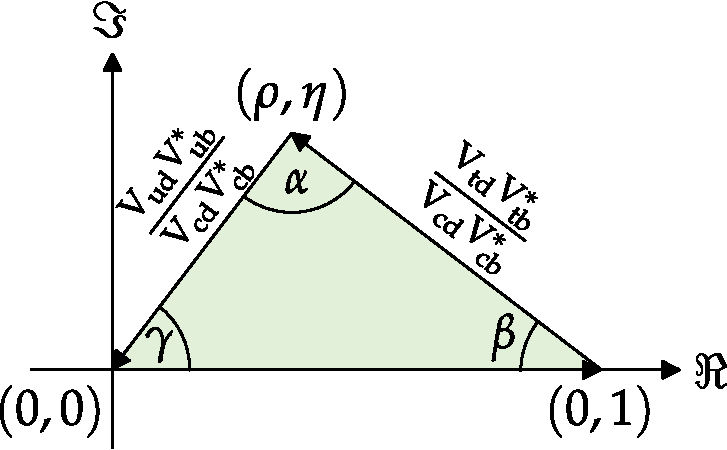
\includegraphics[height=0.25\textwidth]{Triangle2.pdf}} \hfill
\subfloat[Triángulo unitario que se forma para el mesón $\text{B}{}_s^0$.\label{fig_ckmb}]{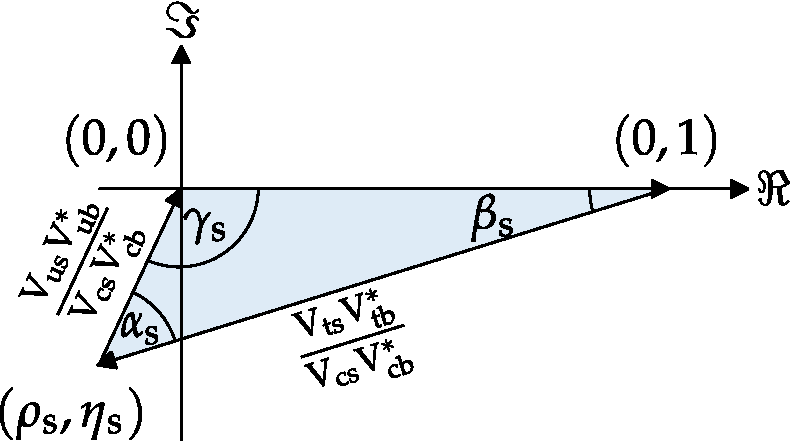
\includegraphics[height=0.25\textwidth]{Triangle1.pdf}} \hfill
%
\caption{Dos de los triángulos que se pueden construir con los elementos de $\vckm$ y la condición de unitariedad. Los triángulos no se encuentran dibujados a escala.}	
\end{figure}


Por la condición de unitariedad se pueden construir diferentes triángulos con la matriz $\vckm$, que son motivo de profundos estudios de precisión del modelo de Kobayashi--Maskawa, entre ellos verificar la unitariedad de esta matriz. Uno de ellos, aunque casi degenerado en rectas, es el reflejado en la Figura \ref{fig_ckmb},
\begin{equation}
 V_{\mathrm{us}} V_{\mathrm{ub}}^* + V_{\mathrm{cs}} V_{\mathrm{cb}}^* + V_{\mathrm{ts}} V_{\mathrm{tb}}^* = 0 
\end{equation}
siendo el menor de los ángulos de este triángulo,
\begin{equation}
	\beta_{\mathrm{s}} =  \text{arg} \left( - \frac{V_{\mathrm{ts}} V_{\mathrm{tb}}^*}{V_{\mathrm{cs}} V_{\mathrm{cb}}^*}   \right)  \label{eq_bs_ckm}
\end{equation}
\color{vero} Asumiendo el \stdmod, y haciendo un ajuste global combinando datos experimentales \cite{ckmfitter1}, se predice el valor  , %cuyo valor se pretende medir por primera vez en esta tesis, y encontrarlo no compatible con cero.
\begin{equation}
	\varphi_{\text{s}}^{\text{SM}} = -2 \beta_{\text{s}} = -36.9\,{}_{-0.8}^{+1.0} \, \text{mrad}. \label{eq_smpredicphis}
\end{equation} \color{norm}
\color{dieg} Cualquier desviación en el valor de $\varphi_{\text{s}}$ (véase \S\ref{sec_phis}), grande o pequeña, es una evidencia de física \bstdmod, haciendo que  sea un excelente observable para estas búsquedas. \color{norm}
%TODO ajuste emph

\subsection{Sistemas de mesones neutros} %%%%%%%%%%%%%%%%%%%%%%%%%%%%%%%%%%%%%%%
\label{sec_neutralmesons}

El número cuántico de sabor es conservado por dos de las interacciones del \stdmod: la electromagnética y la interacción nuclear fuerte. Sin embargo, la interacción débil no conserva el sabor, $\Delta F \neq 0$. Sin pérdida de generalidad, se hará referencia al mesón $\Bs$ como un mesón neutro genérico, puesto que es el \color{vero}estudiado \color{norm} en este trabajo. 

El mesón $\Bs[\mathrm{s\bar b}]$ es un mesón neutro y que tiene por antipartícula al mesón $\Bbs[\mathrm{\bar s b}]$, que es su conjugado en el número cuántico de sabor y también neutro. Ambos pueden convertirse en su antipartícula mediante un proceso denominado oscilaciones mesón--antimesón, propiedad que comparten con todos los mesones neutros pesados. Las oscilaciones de mesones  son posibles en el \stdmod mediante diagramas como los de las Figura \ref{fig_mixing}, y juegan un papel muy importante en la física de sabor, puesto que son muy sensibles a la existencia de nuevas partículas. 

\begin{figure}[H]
\centering
\subfloat{\includegraphics[width=0.48\textwidth,page=3]{feymans.pdf}} \hfill
\subfloat{\includegraphics[width=0.48\textwidth,page=4]{feymans.pdf}} \hfill
\caption{Diagramas de Feynman para la mezcla $\Bs - \Bbs$.} \label{fig_mixing}
\end{figure}


La existencia de la interacción nuclear débil es la que provoca que estos mesones decaigan a otras partículas; sin ella, ambos mesones, $\Bs$ y $\Bbs$, serían un par partícula--antipartícula estable con masa $m_0$, y común a ambos. Así pues, puede decirse que $|\Bs\rangle$ y $|\Bbs\rangle$ son autoestados de las interacciones nuclear fuerte y electromagnética, siendo por tanto $\langle \Bs | \Bbs \rangle = 0$. Sin embargo, una vez se considere el hamiltoniano débil, $\HW$, este provocará que ambos mesones oscilen y decaigan a otros estados \cite{lavoura}.

Se puede escribir el hamiltoniano del sistema en dos partes diferenciadas,
\[\mathcal{H} = \mathcal{H}_0 + \HW ,\]
una que cumple $\Delta F =0$, el operador $\mathcal{H}_0$; y la parte débil, que tratamos como una perturbación, el operador $\HW$.



\subsubsection{Matriz de masa--desintegración}

Como causa del \emph{mixing} de sabor, los mesones neutros están sujetos a oscilaciones partícula--antipartícula, a través de transiciones débiles que cambian el sabor en 2 unidades ($\Delta F = 2$) o bien mediante un estado intermedio (con $\Delta F = 1$). En este caso, la corriente neutra de cambio de sabor (FCNC), que cambia el sabor en 2 unidades, es la responsable de las oscilaciones $\Bs - \Bbs$ ilustradas en los diagramas de Feynman de las Figura \ref{fig_mixing}, y denominados por su topología diagramas de caja. Como resultado de la mezcla de sabor, el estado inicial después de la creación del mesón es una superposición de los estados con $\Bs $ y $\Bbs$,
\[|\psi(t)\rangle = a(t) |\Bs\rangle + b(t) |\Bbs\rangle.\]
%
En la aproximación de Wigner--Weisskopf, que omite las correcciones a la tasa de desintegración exponencial para tiempos muy bajos
%\footnote{El tiempo característico de la interacción fuerte es --.., y nosotros no s interesaremos por estado con $t\gg\tau_S$.} 
o muy altos, el hamiltoniano efectivo del sistema se puede escribir como 
\[\mathcal{H}_{\text{eff}} = \begin{pmatrix}
	M_{11} & M_{12} \\ M_{12}^* & M_{22}
\end{pmatrix} - \frac{i}{2} \begin{pmatrix}
	\Gamma_{11} & \Gamma_{12} \\ \Gamma_{12}^* & \Gamma_{22} 
\end{pmatrix} = \mathbf{M} - \frac{i}{2} \bm{\Gamma} \]
%
\noindent y que no es hermítico\footnote{Sin embargo, tanto $\mathbf{M}$ como $\bm{\Gamma}$ sí son matrices hermíticas ($\mathbf{M} = \mathbf{M}^{\dagger}$ y $\bm{\Gamma} = \bm{\Gamma}^{\dagger}$), verificando además que $\bm{M}=\frac{1}{2} (\mathcal{H}_{\text{eff}} + \mathcal{H}_{\text{eff}}^{\dagger})$ y $\bm{\Gamma} = i(\mathcal{H}_{\text{eff}}-\mathcal{H}_{\text{eff}}^{\dagger})$.}, en cuyo caso los mesones no decaerían y simplemente oscilarían. Este hamiltoniano ha de verificar la ecuación de Schrödinger
\[i \frac{d}{dt} \begin{pmatrix}
	a(t)  \\ b(t)
\end{pmatrix} = \mathcal{H}_{\text{eff}} \begin{pmatrix}
	a(t)   \\ b(t)  
\end{pmatrix}.\]
%
Expandiendo a segundo orden en teoría de perturbaciones \cite{lavoura}, se encuentra que los elementos de las matrices de masa y desintegración son, 
\[M_{ij} = m_0 \delta_{ij} + \langle i | \HW^{\Delta F = 2} | j\rangle  + \sum_k \mathbb{P} \frac{\langle i | \HW^{\Delta F = 1} | k\rangle \langle k | \HW^{\Delta F = 1} | j \rangle }{m_0 - E_k}\]
\[\Gamma_{ij} = 2 \pi \sum_k \delta (m_0 - E_k) \langle i | \HW^{\Delta F = 1} | k\rangle \langle k | \HW^{\Delta F = 1} | j \rangle .\]

En virtud de la invariancia CPT, $M \equiv M_{11} = M_{22}$ y $\Gamma \equiv \Gamma_{11}=\Gamma_{22}$. Los términos no diagonales son responsables del fenómeno de mezcla $\Bs - \Bbs$, que se produce con una frecuencia $\omega$ de oscilación de CKM, donde, para este caso $\Bs$, se involucra al elemento $ V{}_{\text{tb}}^* V{}_{\text{ts}}$. La parte dispersiva $M_{12}$ se corresponde con partículas virtuales de transiciones $\Delta F = 2$ y que están dominadas por partículas muy pesadas en el \stdmod, como el quark \textit{top}. La parte absortiva, $\Gamma_{12}$, se corresponde con transiciones de capa debidas a los modos desintegración que son comunes tanto a mesón como a anti--mesón, $\Delta F = 1$. Ninguno de estos últimos es autoestado de $\mathcal{H}$, puesto que no lo son de $\mathcal{H}_W$ (aunque sí de $\mathcal{H}_0$), por lo que se necesita construir una nueva base. Diagonalizando el hamiltoniano respecto de una base ${\Bs}_{H,L}$, pesado y ligero respectivamente, aparecen estos dos autoestados que no oscilan, simplemente decaen. A cada uno de ellos les corresponde una masa $M_{H,L}$ y una anchura $\Gamma_{H,L}$. Los autovalores son
%
\[\mu_{H,L} = M - i\frac{\Gamma}{2} \pm Q = M - i\frac{\Gamma}{2} \pm \sqrt{\left(M_{12}-i\frac{\Gamma_{12}}{2}\right) \left(M_{12}^*-i\frac{\Gamma_{12}^*}{2}\right)}\]
de donde se sigue que 
\[\Delta m = M_H - M_L =2 \Re (Q) \qquad \Delta \Gamma = \Gamma_L - \Gamma_H = 4 \Im (Q).\]
% $m = \frac{m_H + m_L }{2}$ y $\Gamma = \frac{\Gamma_H + \Gamma_L}{2}$
 
Los autoestados son mezclas de los estados de sabor, con coeficientes complejos, $p$ y $q$, que satisfacen $p^*p + q^*q = 1$,
%
\[| {\Bs}_{H,L} \rangle = p |\Bs \rangle \pm q | \Bbs \rangle \]
%
siendo 
\begin{equation}
\frac{q}{p}  = \pm \sqrt{\frac {M_{12}^*-i\frac{\Gamma_{12}^*}{2}} {M_{12}-i\frac{\Gamma_{12}}{2}} }	.\label{eq_qp_cocient}
\end{equation}



\subsubsection{Evolución temporal} %%%%%%%%%%%%%%%%%%%%%%%%%%%%%%%%%%%%%%%%%%%%%%%%
\label{sec_evotempB}

La evolución temporal de los dos autoestados viene dada por los autovalores,
\[|{\Bs}_{H,L} (t) \rangle  = e^{-i \mu_{H,L}t } |{\Bs}_{H,L} (0)\rangle = e^{-i (m_{H,L} - \frac{1}{2} \Gamma_{H,L})t} |{\Bs}_{H,L} (0)\rangle. \]
Por su parte, la evolución temporal de los estados de sabor, $\Bs$ y $\Bbs$, viene dada por las dos siguientes ecuaciones
\begin{equation}
\begin{split}
|\Bs\rangle  = g_+(t) |\Bs\rangle  + \frac{q}{p} g_-(t) |\Bbs\rangle\\
|\Bbs\rangle = g_+(t) |\Bbs\rangle + \frac{p}{q} g_-(t) |\Bs \rangle
\end{split}	
\end{equation}
%
con la dependencia temporal expresada mediante las funciones
\begin{equation}
\begin{split}
g_{\pm}(t) &=  \frac{1}{2} \left( e^{-iM_Lt} e^{-\frac{\Gamma_L}{2} t} \pm e^{-iM_Ht} e^{-\frac{\Gamma_H}{2} t} \right) \\
& = \frac{1}{2} e^{-im_{\Bs}t} e^{-\frac{\Gamma}{2}t} \left( e^{i\frac{\Delta m}{2}t} e^{-\frac{\Delta \Gamma}{4}t}  \pm e^{-i\frac{\Delta m}{2}t} e^{\frac{\Delta \Gamma}{4}t} \right).	
\end{split} \label{eq_gedete}
\end{equation}
%
%
%
%\[|g_{\pm}(t)|^2 = \frac{e^{-\Gamma t}}{2} \left[ \cosh \frac{\Delta \Gamma t}{2} \pm \cos \Delta m t \right]\]
%\[g_+^* g_-(t) = -\frac{e^{-\Gamma t}}{2} \left[ \sinh \frac{\Delta \Gamma t}{2} \pm i\sin \Delta m t \right] \]
%
%
%TODO change pictures
\begin{figure}[H]
\centering
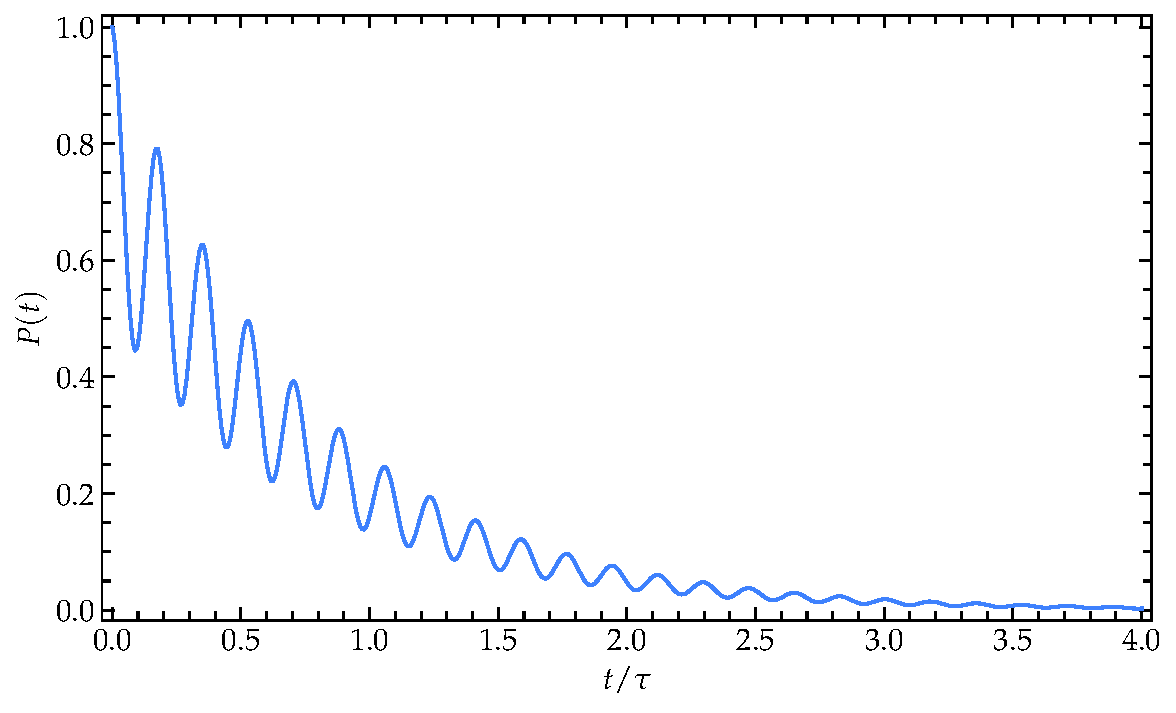
\includegraphics[width=0.48\textwidth]{plots/gpm_total}	 \hfill
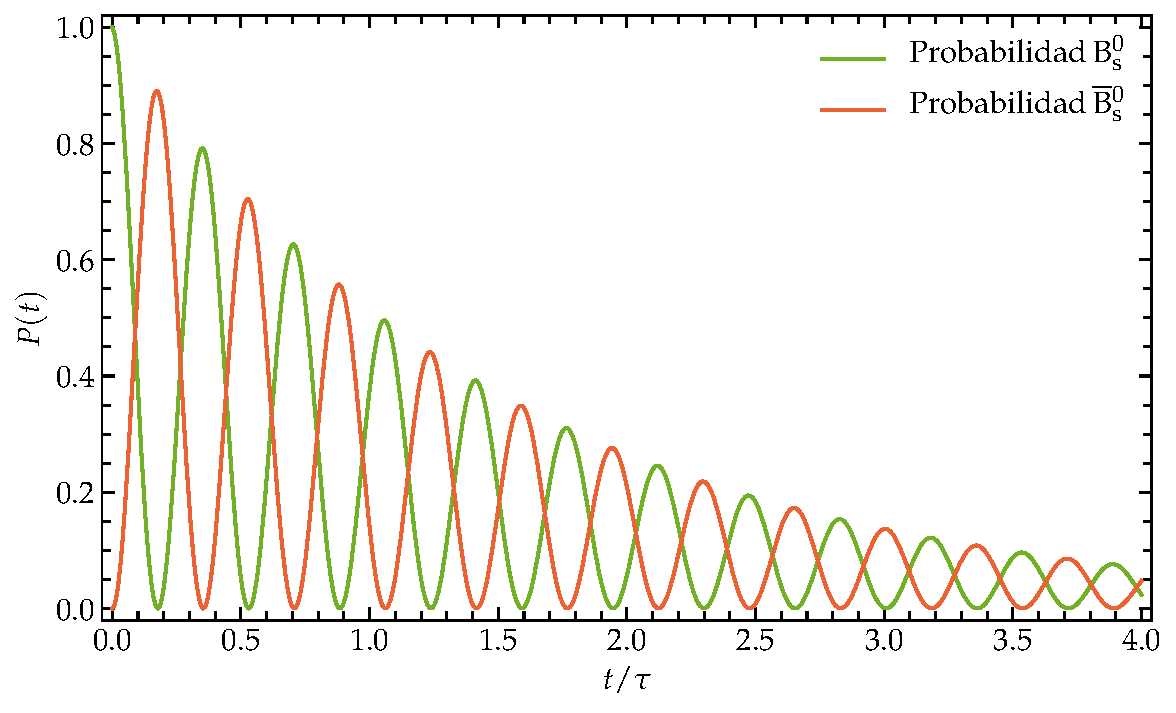
\includegraphics[width=0.48\textwidth]{plots/gpm_bbbar}	 \hfill
\caption{Probabilidad de observar un mesón $\Bs \text{ o } \Bbs$ --- conjuntamente  (izquierda) y separadamente (derecha) --- a tiempo $t$ \color{vero} y para un suceso inicial $\Bs$. \color{norm} }
\end{figure}

Entonces, para un determinado estado final $|f\rangle$ (y su conjugado), existen las cuatro siguientes posibles amplitudes
\begin{equation}
\begin{split}
\mathcal{A}_f = \langle f | \HW | \Bs \rangle \qquad \qquad\mathcal{A}_{\bar f} = \langle \bar f | \HW | \Bs \rangle \\
\overline{\mathcal{A}_f} = \langle f | \HW | \Bbs \rangle \qquad \qquad \overline{\mathcal{A}_{\bar f}} = \langle \bar f | \HW | \Bbs \rangle
\end{split}
\end{equation}
%
\color{vero} y donde se puede definir la cantidad compleja que gobierna las simetrías CP, 
%
\begin{equation}
\lambda_f = \frac{q}{p} \frac{\overline{\mathcal{A}_f}}{\mathcal{A}_f}.
\end{equation}
\color{norm}






\subsection{Violación CP} %%%%%%%%%%%%%%%%%%%%%%%%%%%%%%%%%%%%%%%%%%%%%%%%%%%%%%


\color{vero} La parte teórica \color{norm}  precisa de la existencia de una fase (véase Apéndice \ref{ap_cpvio}), lo que implica en el terreno experimental que esta fase cuántica compleja aparezca y sea medida en procesos de interferencia. Estos procesos han de ser de amplitudes de tamaño similar y que interfieran entre ellas. Si se consideran las secciones eficaces para los procesos $\text{M} \rightarrow f $ y $\overline{\text{M}} \rightarrow \bar f $, se da la siguiente proporcionalidad:
\[\Gamma (\text{M} \rightarrow f )  \sim e^{-\Gamma t} \, |\mathcal{A}_f|^2 \, \left| \frac{p}{q} \right|^2 \qquad	
\overline{\Gamma} (\overline{\text{M}} \rightarrow \bar f )  \sim e^{-\Gamma t} \,  |\overline{\mathcal{A}}_{\bar f}|^2 \, \left| \frac{p}{q} \right|^2.\]
A la vista de las expresiones, para ver cómo la interferencia entre amplitudes se ve reflejada en los módulos cuadrados y dónde podrían estar incluidas las fases que violarían la simetría CP, es útil escribir las amplitudes de la siguiente forma \color{vero}
\begin{equation}
\begin{split}
\mathcal{A}_f & = A_1 e^{i(\delta_1+\varphi_1)}	 + A_2 e^{i(\delta_2+\varphi_2)}	\\
\overline{\mathcal{A}}_{\overline{f}} & = A_1e^{i(\delta_1-\varphi_1)}	 + A_2e^{i(\delta_2-\varphi_2)}	
\end{split}
\end{equation} \color{norm}
donde la cantidad de violación CP vendrá dada por las llamadas fases de violación CP, $\varphi$, que emanan de los términos del lagrangiano que violan CP (es decir, que cambian de signo al aplicarle $\OPcp$). En el SM esto solo puede suceder mediante la interacción débil  y por lo tanto estas fases suelen denominarse fases débiles.  Las fases que conservan CP, $\delta$, provienen de términos del lagrangiano que son invariantes bajo $\OPcp$, y en el SM están típicamente relacionadas con la interacción fuerte, y por ello se denominan fases fuertes o hadrónicas.
Además, para el caso de mesones neutros, como el $\Bs$, es útil definir
\begin{equation}
	M_{12} = |M_{12}|e^{i\varphi_M}, \qquad \Gamma_{12} = |\Gamma_{12}|e^{i\varphi_{\Gamma}}
\end{equation}
%
En la literatura \cite{lavoura}, suelen distinguirse 3 tipos de violación CP ligadas a asimetrías entre amplitudes, $\mathscr{A}$, que se desglosan a continuación.



\subsubsection{Violación CP directa: CPV en la desintegración} %%%%%%%%%%%%%%%%%
\label{sec_CPVdesint}

Cuando las amplitudes de los procesos $A_f$ y $\overline{A}_{\bar f}$ (el proceso conjugado)  son distintas, entonces se tiene violación CP dado que \cite{pdg2018}
\begin{equation*}
\left| \frac{A_f}{\overline{A}_{\bar f}} \right| \neq 1 \qquad \Rightarrow \qquad \mathscr{A} _D = \frac{\overline{\Gamma}-\Gamma}{\overline{\Gamma}+\Gamma}=\frac{ \left| \sfrac{\overline{\mathcal{A}}_{\overline{f}}}{\mathcal{A}_f} \right|^2 -1 }{\left| \sfrac{\overline{\mathcal{A}}_{\overline{f}}}{\mathcal{A}_f} \right|^2 +1}.
\end{equation*}
%
Esta diferencia puede medirse en un proceso de interferencia y ser enorme puesto que 
\begin{equation}
\mathscr{A}_D \propto |A_f|^2 - |\overline{A}_{\overline{f}}|^2 = -4A_1A_2 \sin(\delta_1 - \delta_2) \sin (\varphi_1 - \varphi_2).	\label{eqinferf1}
\end{equation}
\color{vero} Esta \color{norm} es la única fuente de violación CP en sistemas de mesones cargados (puesto que estos no se ven afectados por la mezcla, $\Delta F = 1$).



\subsubsection{Violación CP indirecta: CPV (y TV) en la mezcla} %%%%%%%%%%%%%%%%
\label{sec_CPVmixing}

\color{vero} Se define la violación CP en la mezcla mediante \cite{pdg2018}\color{rem}
\begin{equation}
 \left| \frac{q}{p} \right| \neq 1	\qquad \Rightarrow \qquad \mathscr{A}_M = \frac{\sfrac{d\overline{\Gamma}}{dt}-\sfrac{d\Gamma}{dt}}{\sfrac{d\overline{\Gamma}}{dt}+\sfrac{d\Gamma}{dt}}  =  \frac{1- \left| \sfrac{q}{p} \right|^4}{1+ \left| \sfrac{q}{p} \right|^4},
\end{equation} 
un tipo de violación CP que se ha visto y medido en desintegraciones semileptónicas. Nótese que esta asimetría de tasas de desintegración dependientes del tiempo es, de hecho, no dependiente del tiempo.  \color{norm}

Si se manifiesta esta violación CP, vendría a indicar que en los procesos con $\Delta F = 2$ la mezcla que se produce en las Figuras \ref{fig_mix_a} y \ref{fig_mix_b} es distinta. Un proceso de violación CP en este caso requeriría de contribuciones en \color{vero} la mezcla \color{norm} que son similares en tamaño. Bajo la aproximación $M_{12} \gg \Gamma_{12}$ (válida para el $\Bs$), esta asimetría en desintegraciones de mesones neutros es
\begin{equation}
\mathscr{A}_M \propto \left| \frac{\Gamma_{12}}{M_{12}} \right| \sin (\varphi_M - \varphi_{\Gamma}),	
\end{equation}
aunque se trata de un factor pequeño y difícil de calcular, puesto que involucra \emph{long--distance physics}.



\subsubsection{Violación CP en la interferencia} %%%%%%%%%%%%%%%%%%%%%%%%%%%%%%%
\label{sec_cpvinter}

\begin{wrapfigure}{r}{0.45\textwidth}
\centering
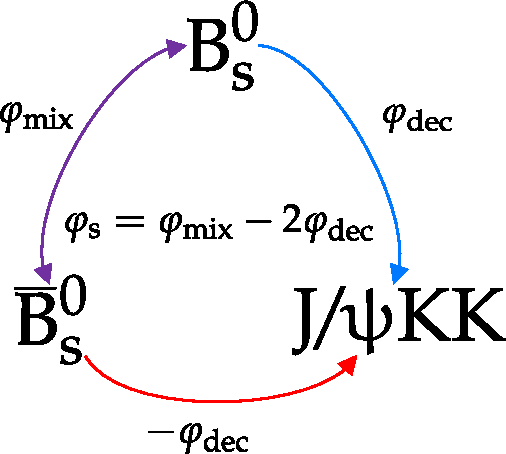
\includegraphics[width=0.3\textwidth]{PhisScheme.pdf}
\caption{Interferencia entre la desintegración directa y la desintegración después de la mezcla.}	\label{fig_oscillatenoscillate}
\end{wrapfigure}
Medir violación CP a través de asimetrías directas (\S \ref{sec_CPVdesint}) o en el \emph{mixing} (\S \ref{sec_CPVmixing}) no es la única forma de acceder a las fases de la matriz $\vckm$. Se puede también medir procesos de interferencia más sutiles donde no haya tanto protagonismo de las fases fuertes\footnote{\color{vero}En la Ecuación (\ref{eqinferf1}), se observa el seno de la diferencia de fases fuertes, que puede ser pequeño en algunos casos; y en dichos casos 'suprime' la posibilidad de observar los fenómenos de interferencia. \color{norm}}.
%
La interferencia puede producirse entre la desintegración del mesón y su oscilación partícula--antipartícula, en el estado entrelazado que se produce antes de la desintegración.
%
La teoría EW es capaz, por sí misma, de convertir espontáneamente un mesón neutro en su antipartícula a través, principalmente, del quark \textit{top}, aunque también de \emph{up} y \emph{charm}, como se observa en las Figuras \ref{fig_mix_a} y \ref{fig_mix_b}: se van intercambiando $\Bs$ y $\Bbs$ con una cierta frecuencia. Si ambos mesones tienen el mismo estado final, $f = \overline{f}$,  entonces estos podrán decaer al estado final habiendo o no oscilado previamente (véase Figura \ref{fig_oscillatenoscillate}).
%
Es posible observar violación CP incluso en ausencia de violación CP directa e indirecta, $|\lambda_f| = 1$. En este caso, $\lambda_f$ es una fase pura, típicamente \cite{pdg2018}, 
\begin{equation}
	\Im(\lambda_f) \neq 0  \,\, \Rightarrow \,\, \mathscr{A}_{\lambda} = \frac{
	\sfrac{d{\Gamma}(\overline{M}\rightarrow f )}{dt}-\sfrac{d\Gamma({M}\rightarrow f )}{dt}}{
	\sfrac{d{\Gamma(\overline{M}\rightarrow f )}}{dt}+\sfrac{d\Gamma({M}\rightarrow f )}{dt}} \propto \Im (\lambda_f) \sin (\Delta m \, t). \label{eq_alanda}
\end{equation}
%
De este modo, la fase medida aquí sería una fase débil, sin influencia de fases hadrónicas.



%%%%%%%%%%%%%%%%%%%%%%%%%%%%%%%%%%%%%%%%%%%%%%%%%%%%%%%%%%%%%%%%%%%%%%%%%%%%%%%%
%%%%%%%%%%%%%%%%%%%%%%%%%%%%%%%%%%%%%%%%%%%%%%%%%%%%%%%%%%%%%%%%%%%%%%%%%%%%%%%%
%%%%%%%%%%%%%%%%%%%%%%%%%%%%%%%%%%%%%%%%%%%%%%%%%%%%%%%%%%%%%%%%%%%%%%%%%%%%%%%%

\bigskip

\begin{center}
	$***$
\end{center}

\medskip

%%%%%%%%%%%%%%%%%%%%%%%%%%%%%%%%%%%%%%%%%%%%%%%%%%%%%%%%%%%%%%%%%%%%%%%%%%%%%%%%
%%%%%%%%%%%%%%%%%%%%%%%%%%%%%%%%%%%%%%%%%%%%%%%%%%%%%%%%%%%%%%%%%%%%%%%%%%%%%%%%
%%%%%%%%%%%%%%%%%%%%%%%%%%%%%%%%%%%%%%%%%%%%%%%%%%%%%%%%%%%%%%%%%%%%%%%%%%%%%%%%

\begin{subappendices}

%\titleformat{\section} 
%  {\normalfont}{\spacedlowsmallcaps\appendixname\ %
%  {\spacedallcaps\thesection}}%
%  {1em}{\spacedallcaps}

%%%%%%%%%%%%%%%%%%%%%%%%%%%%%%%%%%%%%%%%%%%%%%%%%%%%%%%%%%%%%%%%%%%%%%%%%%%%%%%%



%%%%%%%%%%%%%%%%%%%%%%%%%%%%%%%%%%%%%%%%%%%%%%%%%%%%%%%%%%%%%%%%%%%%%%%%%%%%%%%%
\section{Fases de CKM y violación CP}  %%%%%%%%%%%%%%%%%%%%%%%%%%%%%%%%%%%%%%%%%
\label{ap_cpvio}

La fase compleja de la matriz CKM es la única fuente de violación CP que se contempla en el sector electrodébil\footnote{Siendo precisos, puede existir violación CP que provenga de interacciones fuertes, mediante el parámetro de violación CP de QCD (véase Tabla \ref{tab_stdparams}). Sin embargo, este parámetro es muy pequeño e irrelevante en el caso de desintegraciones hadrónicas.} de quarks en el \stdmod. Este mecanismo no permite explicar la gran asimetría materia--antimateria que se observa en el Universo actual, por lo tanto deben existir otros procesos adicionales que dieron lugar a esta composición.

Para ver por qué las fases de $\vckm$ tienen la capacidad de generar violación CP, vamos a suponer una colisión a 2 cuerpos entre quarks libres, que denominaremos genéricamente $a\,b \rightarrow c\,d$.
\begin{figure}[H]
\centering
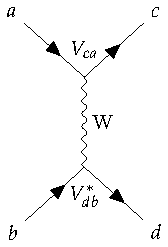
\includegraphics[width = 0.25\textwidth, page =1]{feymans.pdf}
\hspace*{3cm}
\includegraphics[width = 0.25\textwidth, page =2]{feymans.pdf}
\caption{Diagramas de Feynman para el proceso $a\,b \rightarrow c\,d$ (izquierda) y para su proceso conjugado (derecha).}	
\end{figure}
%
En el lagrangiano electrodébil para las corrientes cargadas, es decir, el de la teoría V--A,
todos los términos incluyen al hermítico conjugado. Esto quiere decir que el hamiltoniano de este proceso será $\mathcal{H} \sim M + M^+$, donde $M^+ = M^*$ describe el proceso $cd \rightarrow ab$ (el proceso revertido en el tiempo, es decir, tras la aplicación del operador $\mathcal{T}$). Por tanto, la invariancia CP no consiste en que, al aplicar $\OPcp$ a los espinores involucrados, las amplitudes $M$ y $M_{CP} = \OPcp M$ sean iguales (que sería imposible), sino en que $M_{CP} = M^*$. Es evidente que esto es condición necesaria y suficiente para que 
\[[\OPcp,\mathcal{H}] = 0 \quad  \Leftrightarrow \quad  (\OPcp)^{-1} M (\OPcp) = M^*  .\]
Se debe, por tanto, comparar en detalle $M$, $M_{CP}$ y $M^+$. Para $M$ y su correspondiente $M^+$ se tiene,
\begin{align*}
M & \sim (J_{ca})^{\mu} (J_{bd})_{\mu}^+ \\ & \sim [\bar u_c \gamma^{\mu} (1-\gamma^5) V_{ca} u_a ] \,\, [\bar u_b \gamma_{\mu} (1 -\gamma^5) V_{bd} u_d]^+	\\ & = V_{ca} V_{db}^* [\bar u_c \gamma^{\mu} (1-\gamma^5)  u_a ] \,\, [\bar u_d \gamma_{\mu} (1 -\gamma^5) u_b] \\ M^+ & \sim V_{ca}^* V_{db}[\bar u_a \gamma^{\mu} (1-\gamma^5)  u_c ] \,\, [\bar u_b \gamma_{\mu} (1 -\gamma^5) u_d]
\end{align*}
%
Ahora, al calcular $M_{CP}$ hay que considerar que $u_C = \OPc \overline{u} ^{\top}$ y $\overline{u}_C = - u^{\top} \OPc^{-1}$ \footnote{El operador de conjugación de carga es $\OPc = i \gamma^2 \gamma^0$ y el operador  de paridad es exactamente $\OPp = \gamma^0$.},
luego el conjugado de $ (J_{ca})^{\mu} = \bar u_c \gamma^{\mu} (1-\gamma^5) V_{ca} u_a$ es
\begin{align*}
(J_{ca})_{\phantom{\mu} C}^{\mu} &= -V_{ca} u_c^{\top} C^{-1} \gamma^{\mu} (1-\gamma^5) C \bar{u}_a^{\top}\\ & = + V_{ca} u_c^{\top} [\gamma^{\mu \top} (1- \gamma^5)^{\top}] \bar{u}_a^{\top} \\ &= - V_{ca} \bar{u}_a \gamma^{\mu } (1+ \gamma^5) u_c	
\end{align*}
ahora bien, el operador paridad sobre la regla del vértice, actúa como 
$\OPp^{-1} \gamma^{\mu} (1+ \gamma^5) \OPp = \gamma^{\mu +} (1- \gamma^5)$ y, recordando que $\gamma^{\mu \top} = g^{0\mu} \gamma_{\mu}$ (con $g^{0 \mu} g_{0 \mu} = 1$),
\[(J_{ca})_{\phantom{\mu} CP}^{\mu} = - V_{ca} \bar{u}_a \gamma^{\mu} (1- \gamma^5) u_c.\]
De este modo se obtiene que el elemento de matriz, tras aplicarle el operador $\OPcp$, es
\[M_{CP} = V_{ca}  [\bar{u}_a \gamma^{\mu} (1-\gamma^5)  u_c ] V_{db}^* [\bar{u}_b \gamma_{\mu} (1 -\gamma^5) u_b]\]

La invariancia CP exige, por tanto, que $V_{ca} V_{db}^*$ sea real, ya que solo así se logra $M \leftrightarrows M^+$, para que $\mathcal{H}$ sea invariante; luego la presencia de fases rompe la simetría CP.
%
Entonces, las amplitudes de desintegración para quarks a izquierdas, $\mathcal{A}_f = \langle f |T|i\rangle$, y para antiquarks a derechas, $\overline{\mathcal{A}}_{\bar{f}} = \langle \bar f |T| \bar i\rangle$, pueden ser distinguidas tan 'solo' en una fase. Además, ni la interacción fuerte ni la electromagnética distinguen entre partículas a izquierdas o a derechas, tan solo la interacción débil, que viola paridad, lo hace.

	
\end{subappendices}

%%%%%%%%%%%%%%%%%%%%%%%%%%%%%%%%%%%%%%%%%%%%%%%%%%%%%%%%%%%%%%%%%%%%%%%%%%%%%%%%
%%%%%%%%%%%%%%%%%%%%%%%%%%%%%%%%%%%%%%%%%%%%%%%%%%%%%%%%%%%%%%%%%%%%%%%%%%%%%%%%
%%%%%%%%%%%%%%%%%%%%%%%%%%%%%%%%%%%%%%%%%%%%%%%%%%%%%%%%%%%%%%%%%%%%%%%%%%%%%%%%